
\subsection{Baseline}
We implemented a straightforward version of LambdaMART following Algorithms \ref{alg:lambdamart} and \ref{alg:split} as our optimization baseline. The three core functions in Algorithm \ref{alg:split} are described below.

\mypar{\update}
For each feature, we go through every sample, find out the node and bin index it belongs to, then update the corresponding histogram bin, as illustrated in Figure~\ref{fig:baseline}. The histograms, contiguous in memory, form a matrix where each row is the histogram of one node, and each column represents the same bin of all histograms.

\begin{figure}[h]
  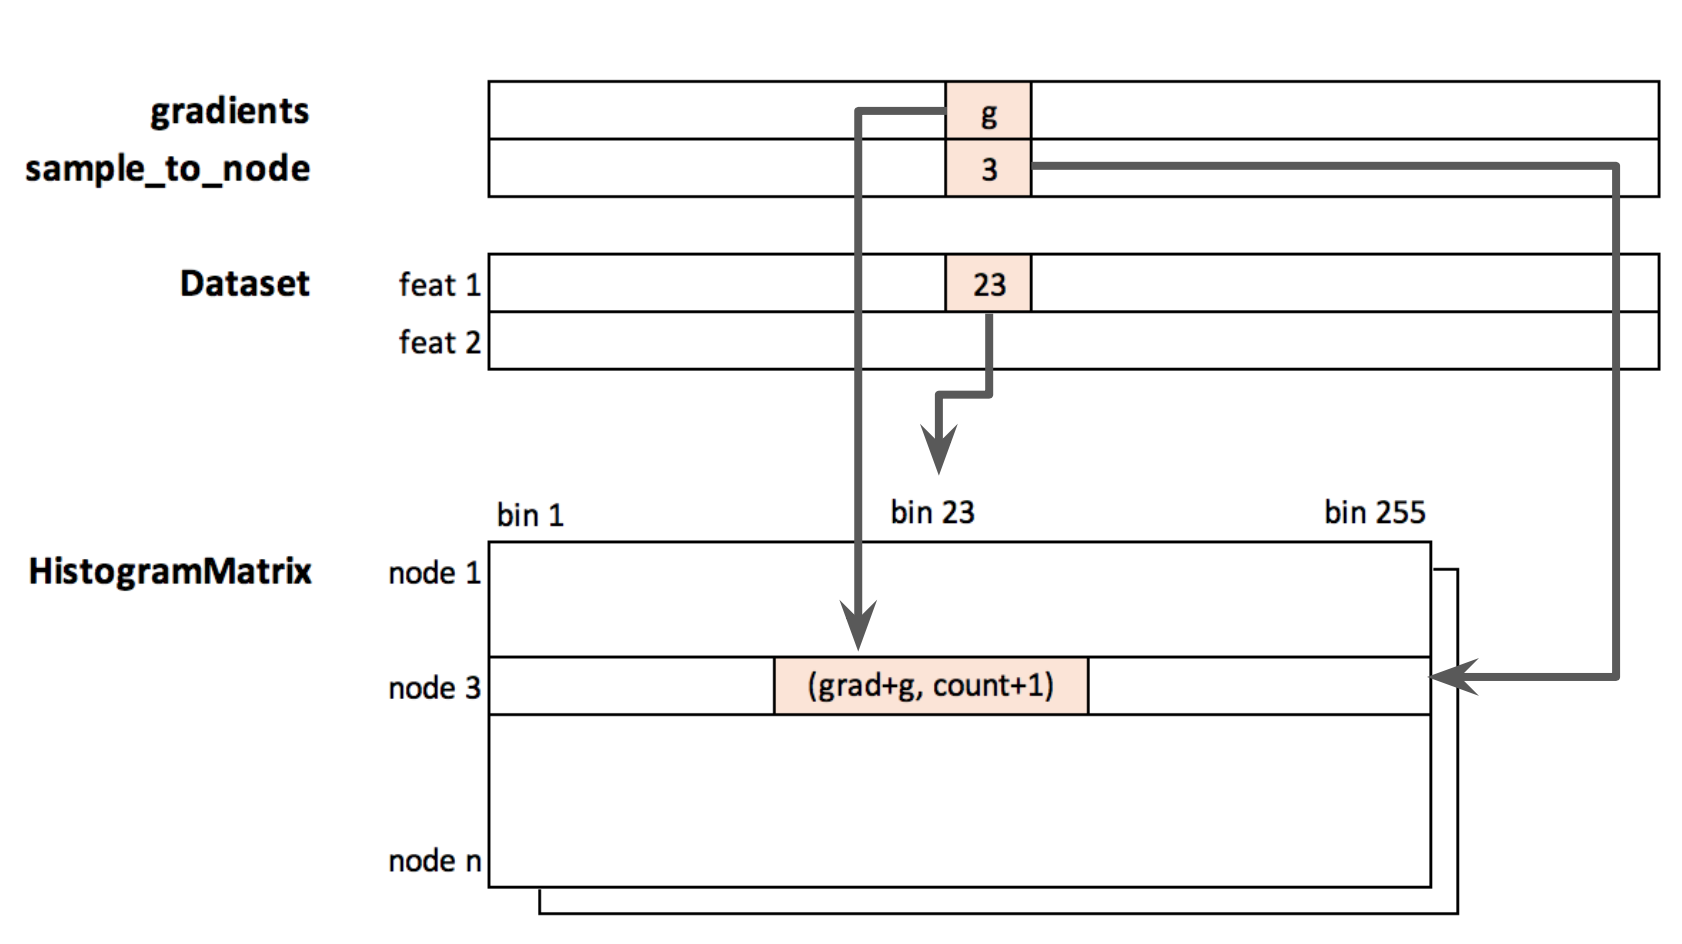
\includegraphics[width=0.47\textwidth]{fig/fig_v0.png}
  \caption{Illustration on updating a histogram bin.}
  \label{fig:baseline}
\end{figure}

Figure~\ref{fig:baseline} also illustrates the lack of locality in \update: \texttt{sample\_to\_node} and \texttt{feat} (a row in \texttt{Dataset}) represent the row and column index of a bin in \texttt{HistogramMatrix}, but both vectors are unordered. As a result, the accesses on \texttt{HistogramMatrix} are fully random, making it hard to parallelize or vectorize. Further, if we consider sorting either vector beforehand to improve locality, we will soon find that the accesses to \texttt{gradients} will become random. Since the size of \texttt{HistogramMatrix} is relatively small and fits into L3 cache, and the size of all other vectors are proportional to the number of samples, we believe it is the best choice to keep all other vectors sequentially accessed, at the cost of randomly accessing \texttt{HistogramMatrix}.

\mypar{\cumulate}
The bins are cumulated to transform the histogram into a suffix sum. After cumulating, each bin contains the sum of all bins starting from it until the last bin. This prepares the sums needed to calculate split gain in \getbestsplit.

\mypar{\getbestsplit}
To get the best split point of one histogram, we go over all bins to find the bin that gives the highest split gain. The right split gain is read directly from the cumulated histogram, while the left gain is calculated from the difference between the total and the right. To ensure no empty nodes are generated, the numbers of samples in both sides also needs to be checked.

\subsection{Feature Blocking}
In \findbestsplit, instead of processing one feature at a time, we block multiple features and process their histograms together.

\mypar{\update}
A crucial observation is that at line \ref{alg:split-grad}-\ref{alg:split-node} in Algorithm \ref{alg:split}, \texttt{gradients} and \texttt{sample\_to\_node} are same for all features of one data sample. 
Thus, we can reduce the accesses to these two vectors by feature blocking. As shown in Fig. \ref{fig:fb}, by processing multiple features at the same time, we can reduce the number of accesses to \texttt{gradients} and \texttt{sample\_to\_node} at the cost of maintaining a bigger HistogramMatrix. 


\begin{figure}[h]
  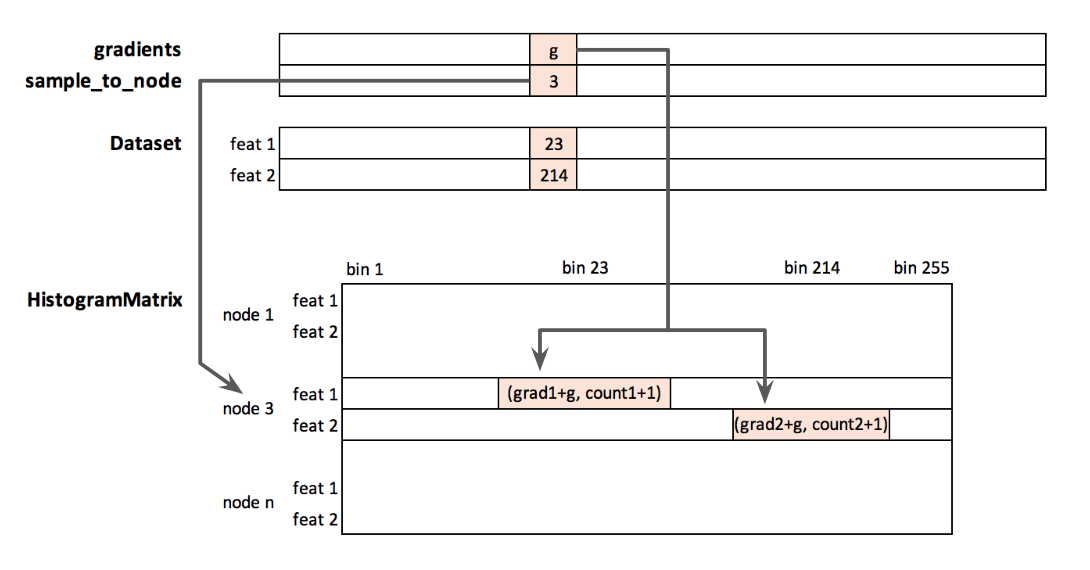
\includegraphics[width=0.47\textwidth]{fig/fig_fb.png}
  \caption{Illustration on feature blocking.}
  \label{fig:fb}
\end{figure}

\mypar{\cumulate}
To cumulate all the $sum\_count$ and $sum\_gradient$ in HistogramMatrix, we noticed that the summation always depends on the previous result and we can take advantage of instruction level parallelism by unrolling and introducing accumulators.
%Furthermore, we notice that there is no dependency across different even if there to increase the ILP
After feature blocking, we can further increase the number of accumulators on different features, and improve the \cumulate.

\mypar{\getbestsplit}
This function cannot directly benefit from feature blocking since the computation for splitGain of different thresholds are not dependent.

\subsection{Vectorization}
% Talk about transposed histogram later
We observed that it is hard to fully utilize the power of SIMD instructions in our case given the dependencies and our data format. 
% To circumvent those issues, we incorporate different strategies while optimizing each function individually. 

\mypar{\update}
\update cannot be vectorized directly as it follows a sequence of bin additions (RAW dependency) into the HistogramMatrix at indexes that cannot be calculated beforehand. Thus, if we vectorize consecutive additions into a single vectorized add, we would end up performing the incorrect operation. Additionally, if we need to perform update on the same bin, doing so would neglect the first three additions. To avoid this, we coupled additions with feature blocking to ensure that we write to different locations in our histogram matrix. 

As the update operations require access to bins at random locations, we make use of \texttt{gather} instructions from AVX-2. In order to use them, we treat addresses as raw integer values and calculate various offsets (using vector operations) to achieve our destination addresses, which are loaded using \texttt{gather}. After updating these values in-register, we store these values back into memory, one-by-one as \texttt{scatter} (store-equivalent of \texttt{gather}) is supported in AVX-512.

\mypar{\cumulate}
Notice that in \cumulate, the bin addition are performed in row major, and bins are added to the one next to them. That is, there are dependencies in every bin addition.
From this observation, it is hard to directly apply AVX vectorization, unless the histogram matrix is transposed and feature blocking is applied, so that the same bin of multiple features can be added at the same time. However, transposing the histogram could worsen the locality of \update as it turns the matrix to bin-major, but the variance of bins is higher than that of nodes. On the other hand, SSE vectorization can still be done since it only load/add one bin (two doubles), and thus avoids the dependency.

%In order to vectorize \cumulate directly, we would need to load bins at the same column but different (consecutive) rows, which introduces unnecessary overhead. To avoid this, we simply transpose our histogram matrix and thus, we need to load bins at same row but consecutive columns. However, since we need to store the results of addition back to memory at each step, we still incur significant overhead.

\mypar{\texttt{get\_best\_splits()}}
Similar to our previous argument, we need to compute values (square of gradients) along the bin-axis and thus, we can only vectorizing one bin (two doubles).
In order to perform vectorization, we combine \texttt{unpacklo/hi} to get a vector of gradinets and counts, and then use SIMD on the two doubles.

%this step would require us to transpose our histogram matrix to bin-major format. However, the \dots.

\subsection{Single-Precision Floating Point Computations}
For our data type optimization, we changed all instances of data type double to float. There are four main data structures that are affected by this change. They are the $scores$ and $gradients$ vectors, storing the sample scores and sample gradients respectively, the $thresholds$ vector that stores the threshold values for each bin, and the HistogramMatrix, which is of the type \texttt{vector\textless{vector}\textless{bin}\textgreater{}\textgreater{}} where bin contains two doubles.

By changing the data type from double to float, we reduced the amount of memory needed by one half. This also means theoretically we can fit twice as much data in each cache line using this optimization compared to our baseline implementation.

\mypar{\texttt{update()}}
From our perf profiling analysis, we found that our program incurs most of its cache misses around the additions of bin's $sum\_count$ and $sum\_gradient$, where the program increments $sum\_count$ by one, obtains the sample gradient from the gradient vector, adds to $sum\_gradient$, and stores both values back to the HistogramMatrix. While addition has the same latency for both doubles and floats, our program will benefit most from having less memory movement with the use of floats.

\mypar{\texttt{cumulate()}}
This function will not benefit much from using floats, because it contains only of sequential add operations of values within the HistogramMatrix.

\mypar{\texttt{get\_best\_splits()}}
This function contains multiple mul and div operations which will directly benefit from using a smaller datatype. In particular, division operation of floats has lower latency and higher throughput compared to that of doubles. Using floats should improve the performance of this function.

\subsection{Sparse Representation for Dataset}
It is a common pattern that the largest bin contains a great portion of samples. Therefore, we can transform the dataset into sparse representation, where every feature only stores the samples that do not fall into the largest bin. When doing histogram \update for a feature, a lot of samples will be skipped, and the information of the largest bin can be recovered by subtracting the sum of all other bins from the total statistics of the corresponding node, which has been stored in the node on its creation. 

This trick is one of the major optimizations in state-of-the-art libraries. However, this optimization reduces the running time by performing fewer flops instead of improving flop per cycle performance. The sparse representation is also hard to integrate with our other optimizations. As a result, we will only implement it and show the running time speedup, and will not include it in our further analysis.